\section{Simon's Problem}
Simon's problem gives an exponential separation between classical and quantum without demanding certain correctness. \\
In some sense, the problem remains hard classically and easy quantumly, even when the oracle is instantiated as a circuit as far as we know: because Shor's algorithm is ``in some sense'' Simon's problem but with the oracle instantiated as a specific circuit. \\
The setup for the problem is the following. For $n \in \N$, let:
\begin{align*}
    \mathcal{D}_0 &:= \{f: \binset \to \binset \mid f \text{ is a bijection}\} \\
    \mathcal{D}_1 &:= \{f: \binset \to \binset \mid \exists! \mathbf{s} \in \binset^n - \{0\}^n, \forall \mathbf{x} \in \binset^n, f(\mathbf{x}) = f(\mathbf{x} \oplus \mathbf{s})\}
\end{align*}
That is, in the case of $\mathcal{D}_1$, if $f(\mathbf{x}) = f(\mathbf{y})$, then $\mathbf{y} \in \{\mathbf{x}, \mathbf{x} \oplus \mathbf{s}\}$, where $\mathbf{s}$ is a unique non-zero bitstring. An example of this is:
\begin{center}
    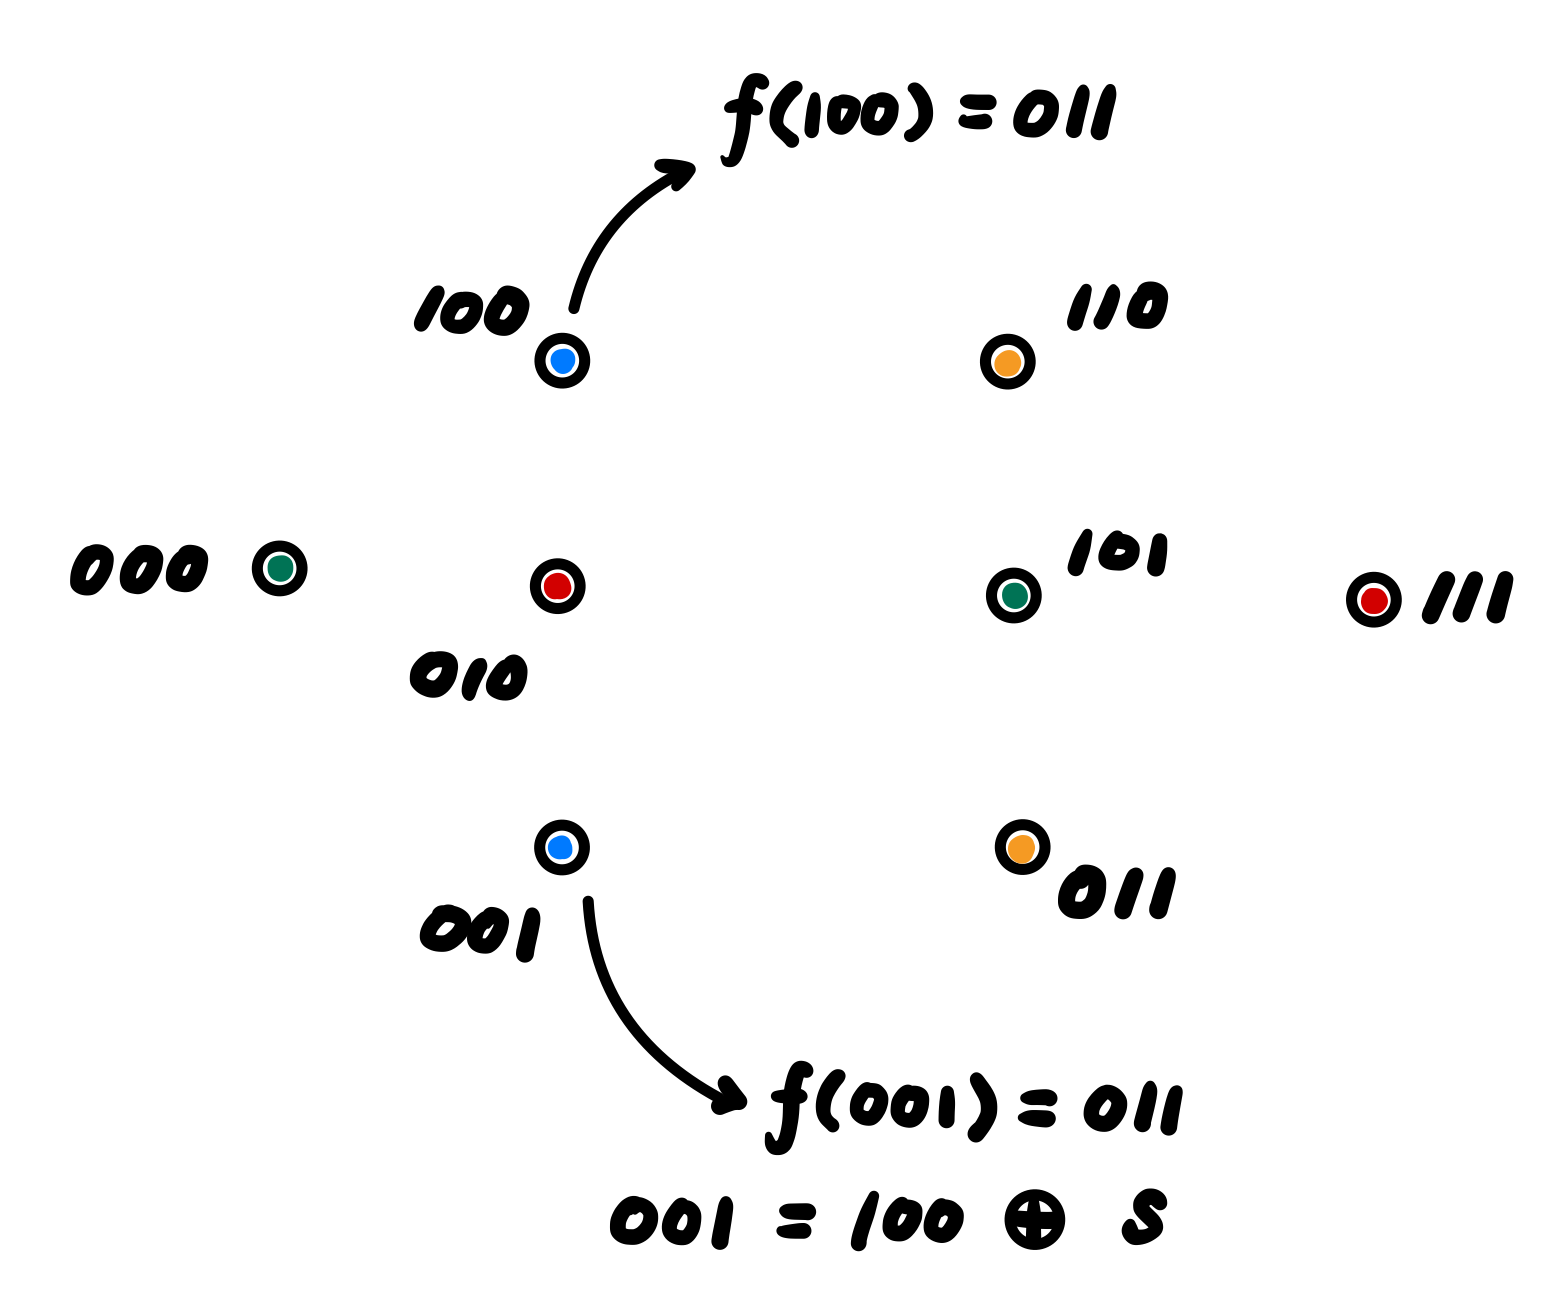
\includegraphics[scale = 0.2]{7/d1_example.png}
\end{center}
where $\mathbf{s} = 101$. We can view this function as a coloring with $2^{n-1}$ colors with each color covering exactly two inputs. Each color represent an output. \\
We want to decide which case $f$ is in, given query access to $f$, \impt{promised} one of the cases hold (but we do not know $\mathbf{s}$). \\
Classically, we need $2^{n-1} + 1$ queries to deterministically solve the problem. When employing a randomized algorithm, the time complexity is $\Theta(\sqrt{2^n})$, which is related to the ``birthday paradox''.

\subsection{Quantum Strategy}
In the quantum case, we only need $\order{n}$ queries and give the correct answer with high probability. The circuit is as follows:
\begin{center}
    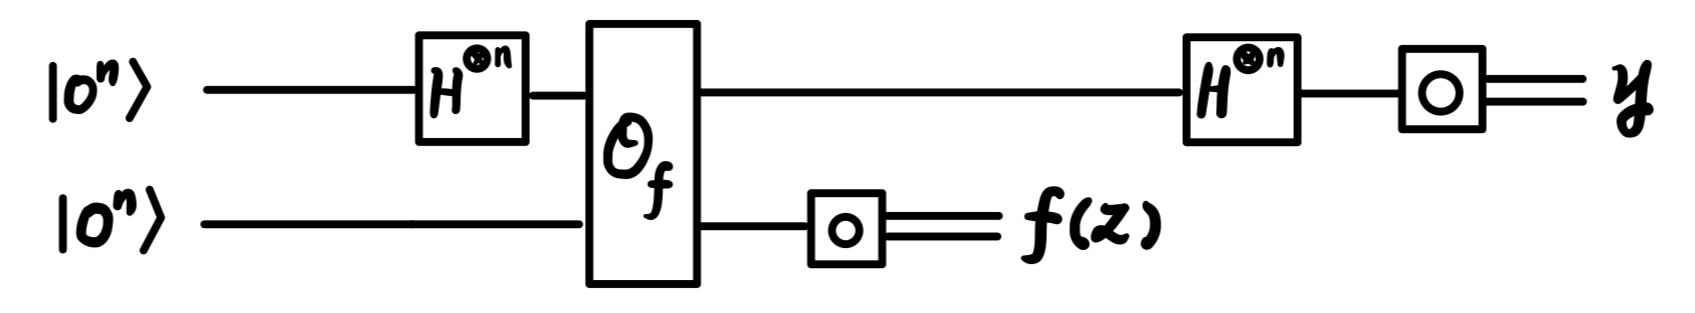
\includegraphics[scale = 0.2]{7/circuit.png}
\end{center}
We measure the last $n$ qubits, and obtain $f(\mathbf{z})$. If $f \in \mathcal{D}_0$, the state of first $n$ qubits collapes to $\ket{\mathbf{z}}$. If $f \in \mathcal{D}_1$, the state of first $n$ qubits collapses to $\frac{1}{\sqrt{2}}(\ket{\mathbf{z}} + \ket{\mathbf{z} \oplus \mathbf{s}})$. \\
Then, after applying $H^n$, if $f \in \mathcal{D}_0$, then we have:
$$\ket{\mathbf{z}} \mapsto \frac{1}{\sqrt{2^n}} \Sumi{\mathbf{y}} (-1)^{\mathbf{y} \cdot \mathbf{z}} \ket{\mathbf{y}}$$
if $f \in \mathcal{D}_1$, then:
$$\frac{1}{\sqrt{2}}(\ket{\mathbf{z}} + \ket{\mathbf{z} \oplus \mathbf{s}}) \mapsto \frac{1}{\sqrt{2^{n+1}}} (\Sumi{\mathbf{y}} (-1)^{\mathbf{y} \cdot \mathbf{z}}(1 + (-1)^{\mathbf{y} \oplus \mathbf{s}})\ket{\mathbf{y}})$$
This means, if we measure the first $n$ qubits, if $f$ is in the first case, each $\mathbf{y}$ has uniform probability of being measured. If $f$ is in the second case, then:
\begin{quote}
    1. $\mathbf{y} \cdot \mathbf{s} \equiv 0 \pmod 2$: $\Prob{\mathbf{y}} = \frac{1}{2^{n - 1}}$. \\
    2. $\mathbf{y} \cdot \mathbf{s} \equiv 1 \pmod 2$: $\Prob{\mathbf{y}} = 0$
\end{quote}
which is uniform over $\{\mathbf{y} \in \binset^n \mid \mathbf{y} \cdot \mathbf{s} \equiv 0 \pmod 2\}$. \\
Repeat the above process $K = \Theta(n) > n$ times to generate $K$ $\mathbf{y}$'s. Collect these $\mathbf{y}$'s into a $K \times n$ matrix:
$$A = \begin{pmatrix}
    \mathbf{y}_1 \\ \mathbf{y}_2 \\ \vdots \\ \mathbf{y}_K
\end{pmatrix}$$
and compute the rank of $A$ over $\F_2$. If the rank is $n$, output $\mathcal{D}_0$, if the rank is $< n$, output $\mathcal{D}_1$.

\begin{definition}
    For a matrix $A$ in $\F_2$, its rank is the \uimpt{minimal non-negative} $d$ such that the set of rows of $A$ can be expressed as 
    $$\{\beta_1 \vecv_1 \oplus \beta_2 \vecv_2 \oplus \cdots \beta_d \vecv_d \mid \beta_1, \beta_2, \dots, \beta_d \in \binset\}$$
    for some zero-one $\vecv_1, \dots, \vecv_d$.
\end{definition}
For example, take $\vecv_1 = (1, 0, 1)$ and $\vecv_2 = (1, 1, 0)$, by iterating through $\beta_1, \beta_2 \in \binset$, we can obtain $3$ non-zero vectors. \\
This gives that the algorithm is always correct in $\mathcal{D}_1$. \\
However, for $f \in \mathcal{D}_0$, we have:
\begin{lemma}
    $$\Prob{\rank A = n} \ge 1 - 2^{n - K}$$
\end{lemma}
Additionally, $\mathbf{s}$ can be computed from $\ker A$.

\newpage